\documentclass[tikz, border = 10pt]{standalone}


\usepackage{newpxtext,newpxmath}   % /upbeta
%\usepackage{fouriernc}            % /otherbeta
\usepackage{amsmath}
\renewcommand{\familydefault}{\sfdefault}
\usepackage{mathastext}

\usetikzlibrary{positioning, quotes, calc, math, arrows.meta, bending, shapes, backgrounds}

\tikzset{
every edge quotes/.style = {fill = white},
every node/.style = {scale = 1.1},
manifest/.style = {rectangle, draw, thin, inner sep = 3pt, minimum width = 1cm,
   minimum height = .85cm, align = center},
latent/.style = {ellipse, draw, thin, inner sep = 3pt, minimum width = 1cm,
   minimum height = .85cm},
residual1/.style = {circle, draw, thin, minimum size = 5mm, inner sep = 1pt},
residual2/.style = {rectangle, minimum width = 0.5pt, minimum height = 1.5mm,
   inner sep = 0pt, outer sep = 0mm},
regression/.style = {-{Stealth[length = 1.5mm]}, thin, shorten > = 1pt, 
   inner sep = 1.5pt, outer sep = 0mm},
covariance/.style={{Stealth[length = 1.5mm]}-{Stealth[length = 1.5mm]}, thin,
   shorten > = 1pt, shorten < = 1pt, inner sep = 1.5pt},
variance/.style={{Stealth[length = 1mm]}-{Stealth[length = 1mm]}, thin,
   shorten > = 1pt, shorten < = 1pt, inner sep = 1pt},
interaction/.style = {-{Stealth[sep = 1pt, length = 1.5mm] . Circle[length = 4pt]},
   thin, shorten > = -2pt},
constant/.style = {draw, thin, inner sep = 1pt, regular polygon,
   regular polygon sides = 3, minimum size = 5mm},
group/.style = {rectangle, inner sep = 2pt, minimum width = 15mm, minimum height = 5mm, 
   align = center}
}

\begin{document}
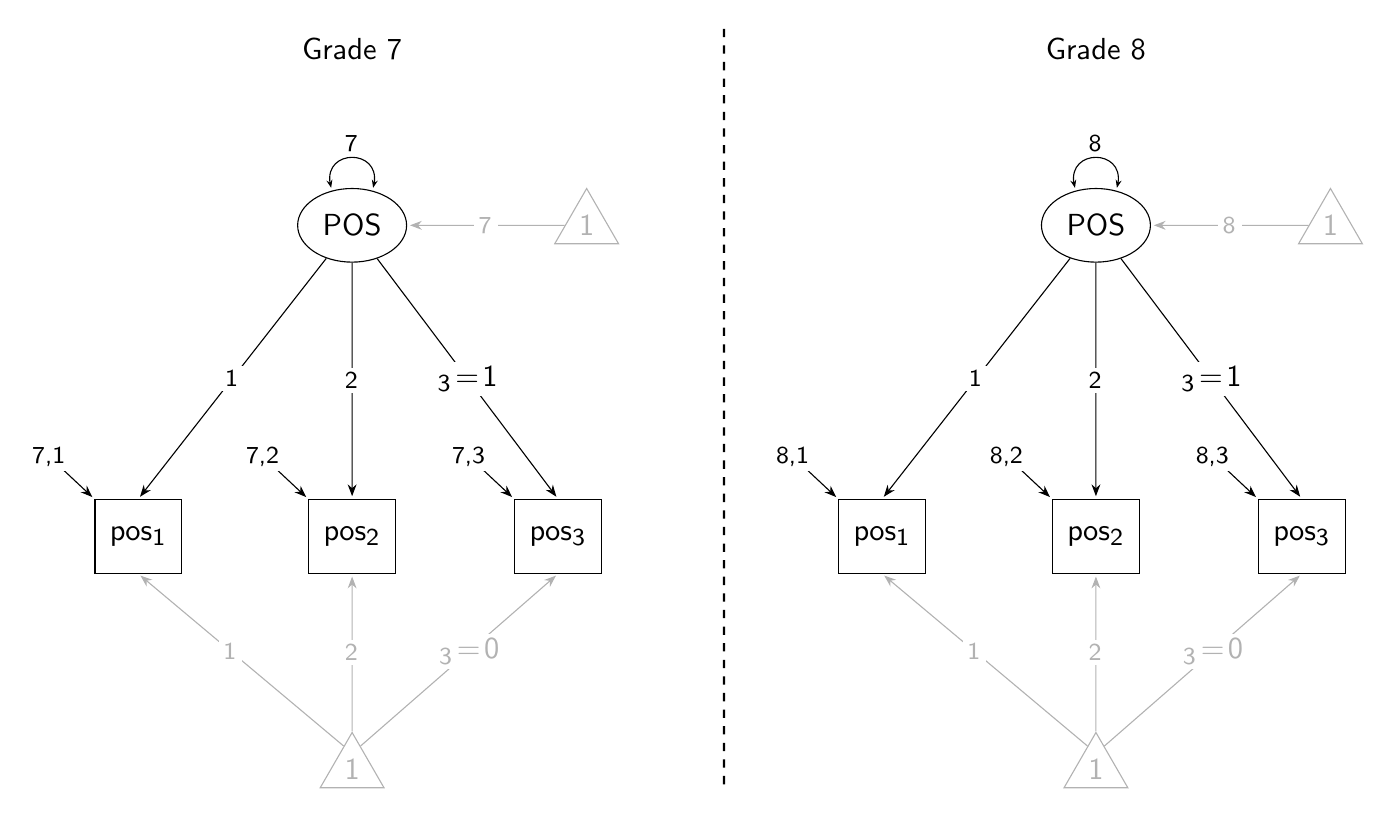
\begin{tikzpicture}

%%%% Grade 7
%% pos manifest
\node [manifest] (pos11) {$pos_1$};
\node [manifest] (pos21) [right = 1.6cm of pos11] {$pos_2$};
\node [manifest] (pos31) [right = 1.5cm of pos21] {$pos_3$};

%% POS latent
\node [latent] (POS1) [above = 3cm of pos21] {$POS$};

%% Loadings
\path [regression] (POS1) edge ["$\uplambda_1$"] (pos11.90);
\path [regression] (POS1) edge ["$\uplambda_2$"] (pos21.90);
\path [regression] (POS1) edge ["$\uplambda_3\!=\!1$"] (pos31.90);

%% Latent variance
\path [variance] (POS1.120) edge ["$\upphi_7$", above, outer sep = 1pt,
   bend left = 110, looseness = 3] (POS1.60);

%% Residuals
\node [residual2] (e11) [above left = .65cm of pos11, xshift = -1mm] {};
\path [regression] (e11) edge ["$\uptheta_{7,1}$", pos = 0] (pos11.north west);

\node [residual2] (e21) [above left = .65cm of pos21, xshift = -1mm] {};
\path [regression] (e21) edge ["$\uptheta_{7,2}$", pos = 0] (pos21.north west);

\node [residual2] (e31) [above left = .65cm of pos31, xshift = -1mm] {};
\path [regression] (e31) edge ["$\uptheta_{7,3}$", pos = 0] (pos31.north west);

%% latent means
\node [constant, black!30] (M11) [right = 2cm of POS1] {1};
\node [constant, black!30] (M21) [below = 2cm of pos21] {1};
\path [regression, black!30] (M11) edge ["$\upkappa_7$"] (POS1);

%% Intercepts
\path [regression, black!30] (M21.110) edge ["$\uptau_1$", pos = 0.55] (pos11.270);
\path [regression, black!30] (M21.90) edge ["$\uptau_2$"] (pos21.270);
\path [regression, black!30] (M21.70) edge ["$\uptau_3\!=\!0$", pos = 0.55] (pos31.270);


%%%% Grade 8
%% pos manifests
\node [manifest] (pos12) [right = 3cm of pos31] {$pos_1$};
\node [manifest] (pos22) [right = 1.6cm of pos12] {$pos_2$};
\node [manifest] (pos32) [right = 1.5cm of pos22] {$pos_3$};

%% POS latent
\node [latent] (POS2) [above = 3cm of pos22] {$POS$};

%% Loadings
\path [regression] (POS2) edge ["$\uplambda_1$"] (pos12.90);
\path [regression] (POS2) edge ["$\uplambda_2$"] (pos22.90);
\path [regression] (POS2) edge ["$\uplambda_3\!=\!1$"] (pos32.90);

%% Latent variance
\path [variance] (POS2.120) edge ["$\upphi_8$", above, outer sep = 1pt,
   bend left = 110, looseness = 3] (POS2.60);

%% Residuals
\node [residual2] (e12) [above left = .65cm of pos12, xshift = -1mm] {};
\path [regression] (e12) edge ["$\uptheta_{8,1}$", pos = 0] (pos12.north west);

\node [residual2] (e22) [above left = .65cm of pos22, xshift = -1mm] {};
\path [regression] (e22) edge ["$\uptheta_{8,2}$", pos = 0] (pos22.north west);

\node [residual2] (e32) [above left = .65cm of pos32, xshift = -1mm] {};
\path [regression] (e32) edge ["$\uptheta_{8,3}$", pos = 0] (pos32.north west);

%% latent means
\node [constant, black!30] (M12) [right = 2cm of POS2] {1};
\node [constant, black!30] (M22) [below = 2cm of pos22] {1};
\path [regression, black!30] (M12) edge ["$\upkappa_8$"] (POS2);

%% Intercepts
\path [regression, black!30] (M22.110) edge ["$\uptau_1$", pos = 0.55] (pos12.270);
\path [regression, black!30] (M22.90) edge ["$\uptau_2$"] (pos22.270);
\path [regression, black!30] (M22.70) edge ["$\uptau_3\!=\!0$", pos = 0.55] (pos32.270);


%%%% Groups
\node (gp1) [above = 1.5cm of POS1] {Grade 7};
\node (gp2) [above = 1.5cm of POS2] {Grade 8};

\node (C1) at ($(gp1)!0.5!(gp2)$) {};
\node (C2) at ($(M21)!0.5!(M22)$) {};
\draw[dashed, thick] ($(C1)!-0.25cm!(C2)$) -- ($(C2)!-0.25cm!(C1)$);

\end{tikzpicture}
\end{document}

